\documentclass[8pt,a4paper,compress]{beamer}

\usepackage{/home/siyer/lib/slides}

\title{Stacks and Queues}
\date{}

\begin{document}
\begin{frame}
\vfill
\titlepage
\end{frame}

\begin{frame}
\frametitle{Outline}
\tableofcontents
\end{frame}

\section{Stacks}
\begin{frame}[fragile]
\pause

A stack is an iterable collection that is based on the last-in-first-out (LIFO) policy

\pause
\bigskip

A data type \lstinline{Stack} that represents a stack
\begin{center}
\begin{tabular}{cc}
method & description \\ \hline
\lstinline$Stack()$ & construct an empty stack $s$ \\
\lstinline$s.isEmpty()$ & is $s$ empty \\
\lstinline$s.push(item)$ & push $item$ on top of $s$ \\
\lstinline$s.pop()$ &  pop and return the item on top of $s$ \\
\lstinline$str(s)$ & a string representation of $s$
\end{tabular} 
\end{center}
\end{frame}

\begin{frame}[fragile]
\pause

\begin{framed}
\tiny stack.py: Definition of \lstinline{Stack} data type.
\end{framed}

\begin{lstlisting}[language=Python]
import stdio

class Stack:
    def __init__(self):
        self._a = []

    def isEmpty(self):
        return len(self._a) == 0

    def push(self, item):
        self._a += [item]

    def pop(self):
        return self._a.pop()

    def __str__(self):
        s = ''
        for item in self._a:
            s = str(item) + ' ' + s
        return s
\end{lstlisting}
\end{frame}

\begin{frame}[fragile]
\pause

\begin{lstlisting}[language=Python]
def main():
    stack = Stack()
    while not stdio.isEmpty():
        item = stdio.readString()
        if item != '-':
            stack.push(item)
        else:
            stdio.write(stack.pop() + ' ')
    stdio.writeln()

if __name__ == '__main__':
    main()
\end{lstlisting}

\pause

\begin{lstlisting}[language={}]
$ more tobe.txt
to be or not to - be - - that - - - is
\end{lstlisting}

\pause

\begin{lstlisting}[language={}]
$ python stack.py < tobe.txt 
to be not that or be
\end{lstlisting}
\end{frame}

\begin{frame}[fragile]
\pause

\begin{framed}
\tiny evaluate.py: Read a fully parenthesized numeric expression from standard input, evaluate it, and write the resulting number to standard output.
\end{framed}

\begin{lstlisting}[language=Python]
import math
import stdio
from stack import Stack

def main():
    ops, values = Stack(), Stack()
    while not stdio.isEmpty():
        token = stdio.readString()
        if   token == '+':    ops.push(token)
        elif token == '-':    ops.push(token)
        elif token == '*':    ops.push(token)
        elif token == 'sqrt': ops.push(token)
        elif token == ')':
            op, value = ops.pop(), ops.pop()
            if   op == '+':    value = values.pop() + value
            elif op == '-':    value = values.pop() - value
            elif op == '*':    value = values.pop() * value
            elif op == 'sqrt': value = math.sqrt(value)
            values.push(value)
        elif token != '(':
            values.push(float(token))
    stdio.writeln(values.pop())

if __name__ == '__main__':
    main()
\end{lstlisting}

\pause

\begin{lstlisting}[language={}]
$ python evaluate.py
( ( 1 + sqrt ( 5.0 ) ) * 0.5 )
<ctrl-d>
1.61803398875
\end{lstlisting}
\end{frame}

\section{Queues}

\begin{frame}[fragile]
\pause

A queue is an iterable collection that is based on the first-in-first-out (FIFO) policy

\pause
\bigskip

A data type \lstinline{Queue} that represents a queue
\begin{center}
\begin{tabular}{cc}
method & description \\ \hline
\lstinline$Queue()$ & construct an empty queue $q$ \\
\lstinline$q.isEmpty()$ & is $q$ empty \\
\lstinline$q.enqueue(item)$ & add $item$ to the end of $q$ \\
\lstinline$q.dequeue()$ &  remove and return the first item of $q$ \\
\lstinline$str(q)$ & a string representation of $q$
\end{tabular} 
\end{center}
\end{frame}

\begin{frame}[fragile]
\pause

\begin{framed}
\tiny queue.py: Definition of \lstinline{Queue} data type.
\end{framed}

\begin{lstlisting}[language=Python]
import stdio

class Queue:
    def __init__(self):
        self._a = []

    def isEmpty(self):
        return len(self._a) == 0

    def enqueue(self, item):
        self._a.insert(0, item)

    def dequeue(self):
        return self._a.pop()

    def __str__(self):
        s = ''
        for item in reversed(self._a):
            s = s + ' ' + str(item)
        return s
\end{lstlisting}
\end{frame}

\begin{frame}[fragile]
\pause

\begin{lstlisting}[language=Python]
def main():
    queue = Queue()
    while not stdio.isEmpty():
        item = stdio.readString()
        if item != '-':
            queue.enqueue(item)
        else:
            stdio.write(queue.dequeue())
            stdio.write(' ')
    stdio.writeln()

if __name__ == '__main__':
    main()
\end{lstlisting}

\pause

\begin{lstlisting}[language={}]
$ more tobe.txt
to be or not to - be - - that - - - is
\end{lstlisting}

\pause

\begin{lstlisting}[language={}]
$ python queue.py < tobe.txt
to be or not to be
\end{lstlisting}
\end{frame}

\begin{frame}[fragile]
\pause

\begin{framed}
\tiny mm1queue.py: Accept float command-line arguments $lamb$ and $mu$, and simulate an M/M/1 queue with arrival rate $lamb$ and service rate $mu$.
\end{framed}

\begin{lstlisting}[language=Python]
import stddraw
import stdrandom
import sys
from histogram import Histogram
from queue import Queue

def main():
    lamb, mu = float(sys.argv[1]), float(sys.argv[2])
    histogram = Histogram(60 + 1)
    queue = Queue()
    stddraw.setCanvasSize(700, 500)
    nextArrival = stdrandom.exp(lamb)
    nextService = nextArrival + stdrandom.exp(mu) 
    while True:
        while nextArrival < nextService:
            queue.enqueue(nextArrival)
            nextArrival += stdrandom.exp(lamb)
        arrival = queue.dequeue()
        wait = nextService - arrival
        stddraw.clear()
        histogram.addDataPoint(min(60, int(round(wait))))
        histogram.draw()
        stddraw.show(20.0)
        if queue.isEmpty():
            nextService = nextArrival + stdrandom.exp(mu)
        else:
            nextService = nextService + stdrandom.exp(mu)

if __name__ == '__main__':
    main()

\end{lstlisting}
\end{frame}

\begin{frame}[fragile]
\pause

\begin{minipage}{200pt}
\begin{lstlisting}[language={}]
$ python mm1queue.py .167 .25
\end{lstlisting}
\end{minipage}%
\hfill
\begin{minipage}{100pt}
\begin{center}
\visible<2->{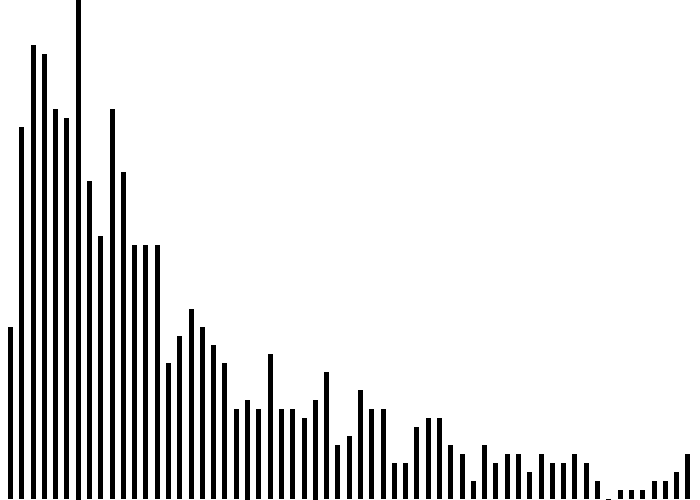
\includegraphics[scale=0.15]{figures/mm1queue1.png}}
\end{center}
\end{minipage}%

\pause
\bigskip

\begin{minipage}{200pt}
\begin{lstlisting}[language={}]
$ python mm1queue.py .167 .2
\end{lstlisting}
\end{minipage}%
\hfill
\begin{minipage}{100pt}
\begin{center}
\visible<3->{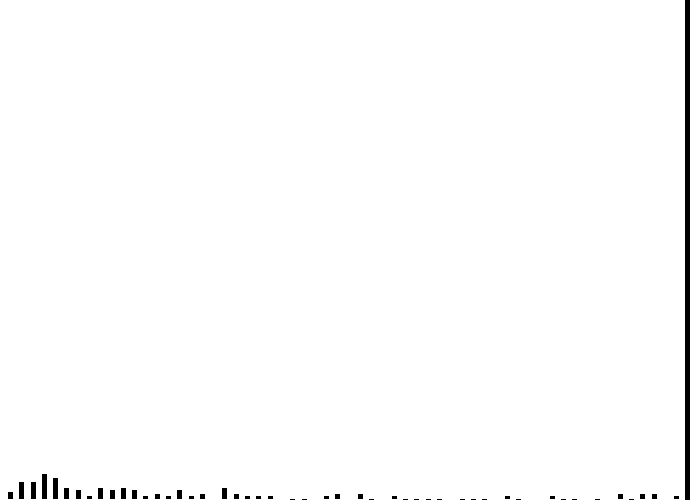
\includegraphics[scale=0.15]{figures/mm1queue2.png}}
\end{center}
\end{minipage}
\end{frame}
\end{document}
